\documentclass{beamer}

% Choose theme 
\usetheme{qrmMMXV}
\usecolortheme{qrmMMXV}

%\usepackage[utf8]{inputenc}

% \usecolortheme{threadless}
\usepackage{mathtools}
\usepackage{xspace}
\usepackage{fancybox}
\usepackage{fancyvrb}
\usepackage{tikz}
\usepackage{pgf}
\usetikzlibrary{arrows,automata}
% \pgfdeclarelayer{background}
% \pgfdeclarelayer{foreground}
% \pgfsetlayers{background,main,foreground}



\newcommand{\qrm}{\texttt{qr\_mumps}\xspace}
\newcommand{\qrs}{\texttt{qr\_starpu}\xspace}
\newcommand{\qrp}{\texttt{qr\_parsec}\xspace}
\newcommand{\spqr}{\texttt{spqr}\xspace}
\newcommand\ignore[1]{{}}

\author{{\bf E.~Agullo}, G.~Bosilca, A.~Buttari, A.~Guermouche and F.~Lopez}
\institute{Universit\'e de Toulouse-IRIT}
\title{Experiments with multifrontal QR using a PTG model}
\subtitle{ANR SOLHAR}
\date{Euro-Par'12}


\makeatletter
\AtBeginPart{%
  \addtocontents{toc}{\protect\beamer@partintoc{\the\c@part}{\beamer@partnameshort}{\the\c@page}}%
}
%% number, shortname, page.
\providecommand\beamer@partintoc[3]{%
  \ifnum\c@tocdepth=-1\relax
    % requesting onlyparts.
    \makebox[6em]{PART #1:} #2
    \vspace{0.5cm}
    \par
  \fi
}
\define@key{beamertoc}{onlyparts}[]{%
  \c@tocdepth=-1\relax
}
\makeatother%

\ifxetex
% if you use xelatex for compiling, then you can set a FreeType font
% like this
\usepackage{fontspec}
% \setmainfont[Mapping=tex-text]{Gill Sans MT Std}
 \setmainfont[Mapping=tex-text]{Bryant Pro}
% \setmainfont[Mapping=tex-text]{Ubuntu}
\let\sfdefault\rmdefault
\fi

\newcommand{\dg}[1]{\textcolor{amgreen}{#1}}
\newcommand{\dr}[1]{\textcolor{amred}{#1}}
\newcommand{\db}[1]{\textcolor{amblu}{#1}}
\newcommand{\dd}[1]{\textcolor{gray!70}{#1}}
\newcommand{\gn}[1]{\textcolor{gray!110}{#1}}
\newcommand{\gs}[1]{\textcolor{gray!50}{#1}}
\newcommand{\gt}[1]{\textcolor{gray!20}{#1}}
\newcommand{\dk}[1]{\textcolor{black}{#1}}

\usepackage[procnames]{listings}
\lstset{ %
  backgroundcolor=\color{gray!5},   % choose the background color; you must add \usepackage{color} or \usepackage{xcolor}
  basicstyle=\tt\footnotesize,      % the size of the fonts that are used for the code
  breakatwhitespace=false,          % sets if automatic breaks should only happen at whitespace
  breaklines=true,                  % sets automatic line breaking
  captionpos=b,                     % sets the caption-position to bottom
  commentstyle=\color{amdove},      % comment style
  extendedchars=true,               % lets you use non-ASCII characters; for 8-bits encodings only, does not work with UTF-8
  frame=single,                     % adds a frame around the code
  keepspaces=true,                  % keeps spaces in text, useful for keeping indentation of code (possibly needs columns=flexible)
  keywordstyle=\color{amblu},       % keyword style
  procnamestyle=\color{amred},       % procedures style
  language=[95]fortran,             % the language of the code
  numbers=none,                     % where to put the line-numbers; possible values are (none, left, right)
  numbersep=5pt,                    % how far the line-numbers are from the code
  numberstyle=\tiny\color{gray!20}, % the style that is used for the line-numbers
  rulecolor=\color{amgreen},          % if not set, the frame-color may be changed on line-breaks within not-black text (e.g. comments (green here))
  showspaces=false,                 % show spaces everywhere adding particular underscores; it overrides 'showstringspaces'
  showstringspaces=false,           % underline spaces within strings only
  showtabs=false,                   % show tabs within strings adding particular underscores
  stepnumber=2,                     % the step between two line-numbers. If it's 1, each line will be numbered
  stringstyle=\color{amdove},       % string literal style
  tabsize=2,                        % sets default tabsize to 2 spaces
  title=\lstname,                    % show the filename of files included with \lstinputlisting; also try caption instead of title
  procnamekeys={call}
}


\graphicspath{{../SOLHAR/Reunion_Lyon_0314/}{../SOLHAR/Kickoff_1113/}{../../Papers/SIAM_qrm/}{../SOLHAR/Reunion_Lyon_0314/}{../EuroPar2013/}}


\begin{document}

\begin{frame}[t,plain]
\titlepage

\end{frame}


\part{Context of the work}

%% \begin{frame}[plain]
%%   \partpage
%% \end{frame}

%% \begin{frame}{Runtime systems}
%%   \begin{columns}
%%     \begin{column}{0.45\textwidth}
%%       \center
%%       \only<1>{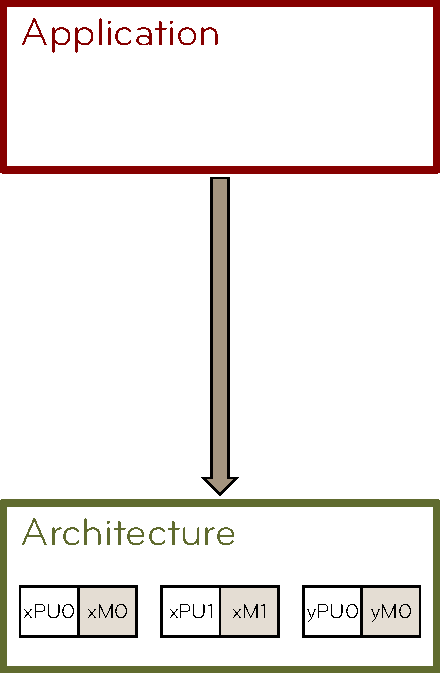
\includegraphics[width=\textwidth]{figures/rt_layers1}}%
%%       \only<2->{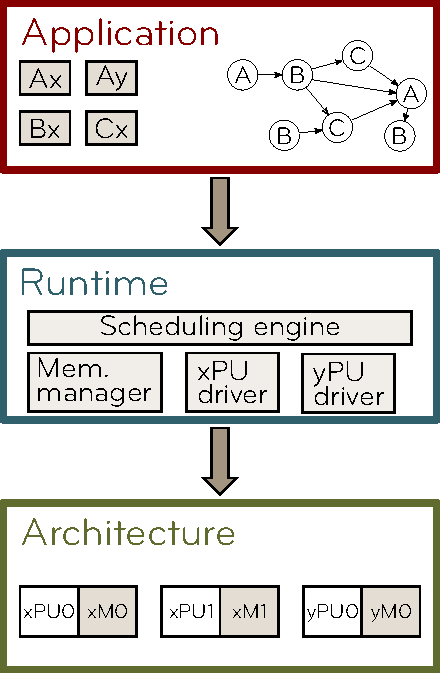
\includegraphics[width=\textwidth]{figures/rt_layers2}}%
%%     \end{column}
%%     \begin{column}{0.55\textwidth}
%%       \begin{itemize}
%%       \item<1->The classical approach is based on a mixture of
%%         technologies (e.g., MPI+OpenMP+CUDA) which
%%         \begin{itemize}
%%         \item requires a big programming effort
%%         \item is difficult to maintain and update
%%         \item is prone to (performance) portability issues
%%         \end{itemize}
%%       \item<2-> runtimes provide an abstraction layer that hides the
%%         architecture details
%%       \item<3-> the workload is expressed as a DAG of tasks where the dependencies are
%%         \begin{itemize}
%%         \item<3-> defined explicitly
%%         \item<3-> defined through rules
%%         \item<3-> automatically inferred
%%         \end{itemize}
%%       \end{itemize}
%%     \end{column}
%%   \end{columns}
%% \end{frame}



%% \begin{frame}{The STF model}

%%   \begin{columns}
%%     \begin{column}{0.6\textwidth}
%%       \begin{block}{Sequential code}
%%         \texttt{sub\_a(x,y); \gn{// R and W x and y}}\\
%%         \texttt{sub\_b(x); ~~\gn{// R x} }\\
%%         \texttt{sub\_c(y); ~~\gn{// R y} }\\
%%         \texttt{sub\_d(x,y); \gn{// R and W x and y}}\\
%%       \end{block}

%%       \vspace{0.5cm}

%%       \begin{exampleblock}{Equivalent STF code}
%%         \uncover<2->{\texttt{\alert{submit}(sub\_a,x:\alert{RW},y:\alert{RW});}}

%%         \uncover<3->{\texttt{\alert{submit}(sub\_b,x:\alert{R});              }}

%%         \uncover<4->{\texttt{\alert{submit}(sub\_c,y:\alert{R});              }}

%%         \uncover<5->{\texttt{\alert{submit}(sub\_d,x:\alert{RW},y:\alert{RW});}}
%%       \end{exampleblock}
%%     \end{column}
%%     \begin{column}{0.4\textwidth}
%%       \begin{tikzpicture}[->,>=stealth',shorten >=1pt,auto,node distance=2.8cm,
%%         semithick]
%%         \tikzstyle{every state}=[fill=gray,draw=none,text=white]

%%         \uncover<2->{\node[state]     (A) at (2,5)  {\texttt{sub\_a}};}
%%         \uncover<3->{\node[state]     (B) at (1,3)  {\texttt{sub\_b}};}
%%         \uncover<4->{\node[state]     (C) at (3,3)  {\texttt{sub\_c}};}
%%         \uncover<5->{\node[state]     (D) at (2,1)  {\texttt{sub\_d}};}

%%         \uncover<3->{\path (A) edge  (B); }
%%         \uncover<4->{\path (A) edge  (C); }
%%         \uncover<5->{\path (B) edge  (D); }
%%         \uncover<5->{\path (C) edge  (D); }
%%       \end{tikzpicture}
%%     \end{column}
%%   \end{columns}

%%   \vspace{0.5cm}

%%   \uncover<6->{\texttt{sub\_b} and \texttt{sub\_c} can be executed in \alert{parallel}.}
%%   \uncover<7->{ Actually, \texttt{sub\_d} also because the
%%     \alert{anti-dependency} can be easily resolved with a copy}
%% \end{frame}




\part{The multifrontal QR method}

\begin{frame}[plain]
  \partpage
\end{frame}


\section{The multifrontal QR method}

\begin{frame}{The Multifrontal QR method}
  \begin{overlayarea}{\textwidth}{1cm}
    \only<1>{The multifrontal QR factorization is guided by a graph called
      \alert{\it elimination tree}:}%
    \only<2->{The tree is traversed in \db{topological order} (i.e., bottom-up)
      and, at each node, two operations are performed:}%
  \end{overlayarea}

  \vspace{0.2cm}

  \begin{columns}
    \begin{column}{0.6\textwidth}
      \begin{overlayarea}{\textwidth}{6cm}
        \only<1>{\begin{itemize}
          \item each node is associated with a relatively small
            \alert{dense} matrix called \db{frontal matrix} (or
            \db{front}) containing k pivots to be eliminated along
            with all the other coefficients concerned by their
            elimination
          \end{itemize}}\only<2->{
          \begin{itemize}
          \item<2-> \alert{assembly}: coefficients from the original
            matrix associated with the pivots and  \alert{\it
              contribution blocks} produced by the treatment of the child
            nodes are \alert{stacked}  to form the frontal matrix
          \item<3-> \alert{factorization}: the $k$ pivots are eliminated
            through a complete QR factorization of the frontal matrix. As a
            result we get:
            \begin{itemize}
            \item part of the global $R$ and $Q$ factors
            \item a triangular \db{\it contribution block} that will be
              assembled into the father's front
            \end{itemize}
          \end{itemize}}
      \end{overlayarea}
    \end{column}
    \begin{column}{0.4\textwidth}
      \begin{center}
      \only<1>{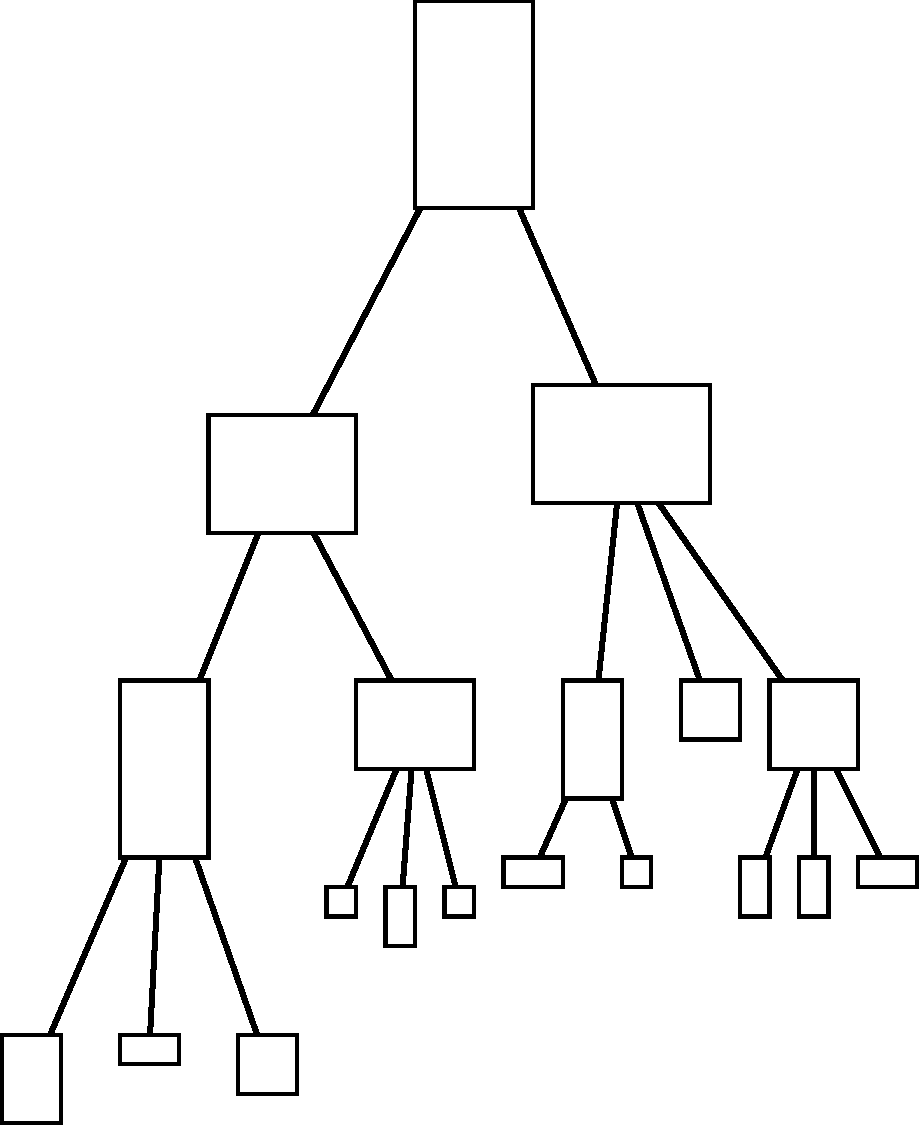
\includegraphics[width=\textwidth]{figures/etree}}%
      \only<2>{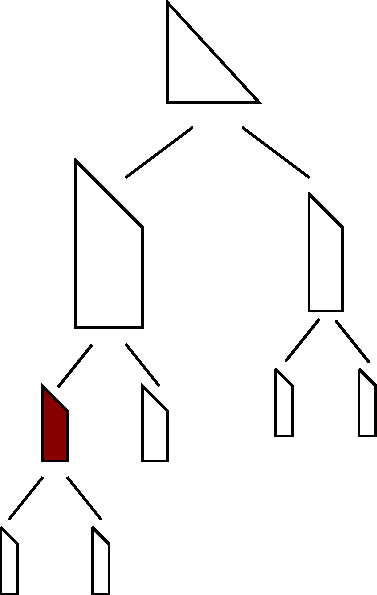
\includegraphics[width=\textwidth]{figures/etree2}}%
      \only<3->{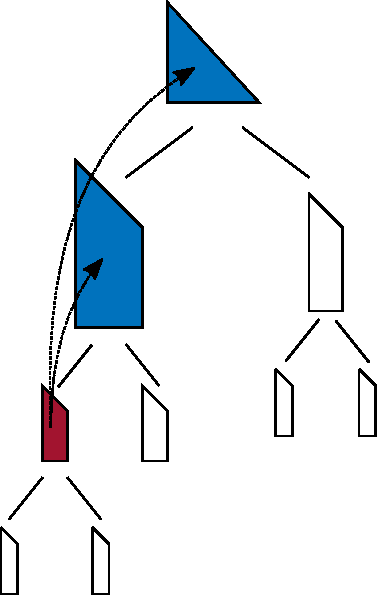
\includegraphics[width=\textwidth]{figures/etree3}}%
      \end{center}
    \end{column}
  \end{columns}


\end{frame}

\begin{frame}{The Multifrontal QR method}
  Notable differences with multifrontal LU:
  \begin{itemize}
  \item \db{fronts are rectangular}, either over or under-determined
  \item \db{assembly operations are just copies} (with lots of indirect
    addressing) and not sums. They can thus be done in any order (like
    in LU) but also in parallel (most likely not efficient because of
    false sharing issues)
  \item \db{fronts are not full}: they have a staircase structure. The
    zeroes in the lower-leftmost part can be ignored. This irregular
    structure makes the modeling of performance rather difficult
  \item \db{fronts are completely factorized} and not just partially. This
    makes the overall size of factors bigger and thus the active
    memory consumption less sensitive to the tree traversal
  \item \db{contribution blocks are trapezoidal} and note square
  \end{itemize}

\end{frame}

\begin{frame}{The Multifrontal QR method: parallelism}

  In the multifrontal methods we can distinguish two sources of
  parallelism:

  \vspace{0.2cm}

  \begin{columns}
    \begin{column}{0.5\textwidth}

      \begin{block}{Tree parallelism}
        Frontal matrices located in independent branches in the
        tree can be processed in parallel
      \end{block}
      
      \begin{block}{Node parallelism}
        Large frontal matrices factorization may be performed in parallel
        by multiple threads
      \end{block}
    \end{column}
    \begin{column}{0.5\textwidth}
      \begin{center}
        \includegraphics[width=0.5\textwidth]{figures/simpletree}
      \end{center}
    \end{column}
  \end{columns}

\end{frame}

\part{The Multifrontal QR method in \qrm}

\begin{frame}[plain]
  \partpage
\end{frame}

\begin{frame}{Parallelism in \qrm: a new approach}

  Our baseline is the approach used in \alert{\qrm} where the
  workload is expressed as a \alert{DAG} of tasks defined through a
  \alert{1D Block-column} partitioning

  \begin{center}
    \includegraphics[width=0.75\textwidth]{figures/dag}
  \end{center}

  In \qrm threading is implemented through OpenMP and scheduling of
  tasks is done ``by hand''

\end{frame}

\begin{frame}{Parallelism: a new approach}
  The \db{scheduling} is performed by a \db{finely-tuned, hand-written code}

  \begin{itemize}
  \item[\db{$\blacktriangle$}] the fine-grained decomposition and the
    asynchronous/dynamic scheduling deliver high concurrency and much
    better performance compared to the classical approach (SPQR)
  \item[\dr{$\blacktriangledown$}] the scheduler is not scalable (the search
    for ready tasks in the DAG is inefficient)...
  \item[\dr{$\blacktriangledown$}] ... extremely difficult to maintain...
  \item[\dr{$\blacktriangledown$}] ... and not really portable
  \end{itemize}

  \vspace{1cm}

\end{frame}

%% \begin{frame}{Parallelism in \qrm: a new approach}

%%   \begin{columns}
%%     \begin{column}{0.5\textwidth}
%%       \begin{block}{\parbox[c][0.4cm]{1.0\linewidth}{Classical approach (SPQR)}}
%%         \begin{minipage}[c][7cm]{1.0\linewidth}
%%           \begin{itemize}
%%           \item separate branches (coarse granularity) are treated
%%             concurrently with some threading mechanism
%%           \item each front is processed using multithreaded BLAS
%%           \end{itemize}
%%           % Coarse grained parallelism (front-wise) plus multithreaded
%%           % BLAS:
%%           This approach
%%           \begin{itemize}
%%           \item requires complex performance modeling
%%           \item suffers from heavy synchronizations
%%           \item is poorly portable
%%           \end{itemize}
%%         \end{minipage}
%%       \end{block}
%%     \end{column}
%%     \begin{column}{0.5\textwidth}
%%       \begin{alertblock}{\parbox[c][0.4cm]{1.0\linewidth}{\qrm}}
%%         \begin{minipage}[c][7cm]{1.0\linewidth}
%%           fine-grained, data-flow parallel approach
%%           \begin{itemize}
%%           \item \underline{ fine granularity}: tasks are not defined as operations on
%%             fronts but as operations on portions of fronts defined by a 1-D
%%             partitioning
%%           \item \underline{ data flow parallelism}: tasks are scheduled dynamically based
%%             on the dependencies between them
%%           \end{itemize}
%%         \end{minipage}
%%       \end{alertblock}
%%     \end{column}
%%   \end{columns}
  
%% \end{frame}

\begin{frame}{Add new features in \qrm}

  We want to develop the following features in
  \qrm:

  \begin{itemize}
  \item \db{2D partitioning} of frontal matrices (finer granularity
    allowing better parallelism) as 1D partitioning may not be adapted
    \begin{itemize} 
    \item most fronts are overdetermined
    \item the problem is mitigated by concurrent front factorizations
    \item[\dg{$\blacktriangle$}]  \uncover<2->{more concurrency}
    \item[\dr{$\blacktriangledown$}]  \uncover<2->{more complex dependencies, more tasks} 
    \end{itemize}
  \item Exploit \db{GPUs}
    \begin{itemize}
    \item[\alert{$\blacktriangledown$}] \uncover<2->{memory transfers, CUDA kernels management} 
    \end{itemize}      
  \item \db{Memory-aware} algorithms (perform factorization under a given
    memory constraint)
  \item \db{Distributed} memory architectures
    \begin{itemize}
    \item[\alert{$\blacktriangledown$}] \uncover<2->{MPI layer} 
    \end{itemize}      
  \end{itemize}

  \begin{center}
    \uncover<2>{  All these problems may be overcome by \alert{using runtime system}}
  \end{center}

\end{frame}

%% \begin{frame}{2D partitioning + CA front factorization}
%%   1D partitioning is not good for (strongly)
%%   \db{overdetermined} matrices:
%%   \begin{itemize}
%%   \item[\dr{$\blacktriangledown$}] most fronts are overdetermined
%%   \item[\dg{$\blacktriangle$}] the problem is mitigated by
%%     concurrent front factorizations
%%   \end{itemize}


%%   \uncover<2>{ 

%%     Thanks to the simplicity of programming models available in
%%     runtime systems it is possible to plug in \alert{2D methods} for
%%     factorizing the frontal matrices with a relatively moderate effort
%%     \begin{itemize}
%%     \item 2D block partitioning (not necessarily square)
%%     \item flat, binary (communication avoiding) or hybrid panel
%%       reduction trees
%%     \item[\dg{$\blacktriangle$}] more concurrency
%%     \item[\dr{$\blacktriangledown$}] more complex dependencies
%%     \item[\dr{$\blacktriangledown$}] many more tasks
%%     \item[\dr{$\blacktriangledown$}] more sensitive to runtime overhead
%%     \end{itemize}
%%   }


%% \end{frame}

\part{STF vs PTG models}

\begin{frame}[plain]
  \partpage
\end{frame}

%% \begin{frame}{Runtime systems}
%%   \begin{columns}
%%     \begin{column}{0.45\textwidth}
%%       \center
%%       \only<1>{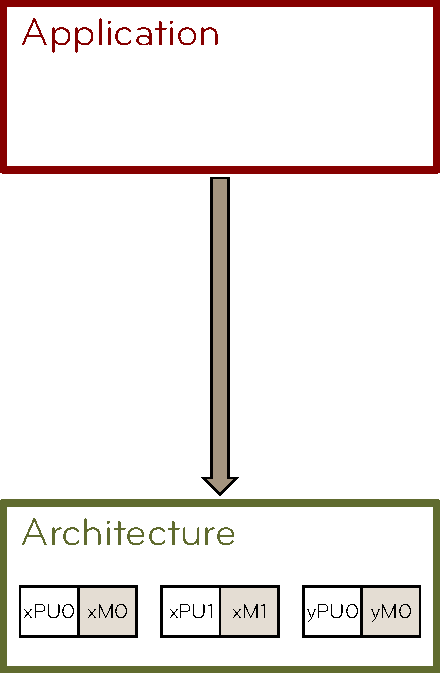
\includegraphics[width=\textwidth]{figures/rt_layers1}}%
%%       \only<2->{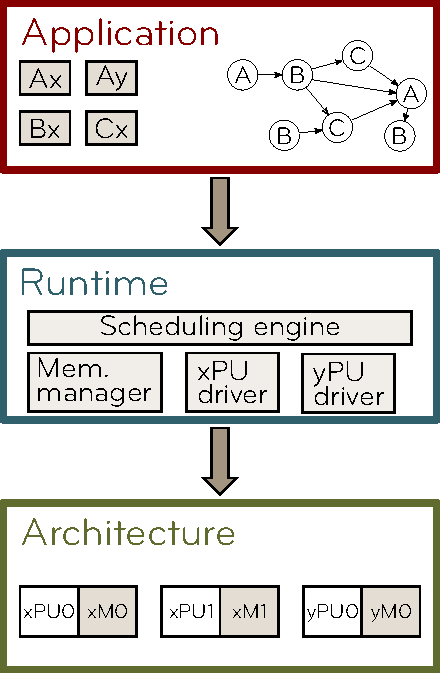
\includegraphics[width=\textwidth]{figures/rt_layers2}}%
%%     \end{column}
%%     \begin{column}{0.55\textwidth}
%%       \begin{itemize}
%%       \item<1->The classical approach is based on a mixture of
%%         technologies (e.g., MPI+OpenMP+CUDA) which
%%         \begin{itemize}
%%         \item requires a big programming effort
%%         \item is difficult to maintain and update
%%         \item is prone to (performance) portability issues
%%         \end{itemize}
%%       \item<2-> runtimes provide an abstraction layer that hides the
%%         architecture details
%%       \item<3-> the workload is expressed as a DAG of tasks where the dependencies are
%%         \begin{itemize}
%%         \item<3-> defined explicitly
%%         \item<3-> defined through rules
%%         \item<3-> automatically inferred
%%         \end{itemize}
%%       \end{itemize}
%%     \end{column}
%%   \end{columns}
%% \end{frame}

\begin{frame}{STF vs PTG models}

  %% \begin{block}{The Sequential Task Flow (STF) model in StarPU:}
  The \alert{Sequential Task Flow} (STF) model in StarPU:
    \begin{itemize}
    \item The parallel corresponds to the sequential one except that
      operations are not executed but \db{submitted} to the system in
      the form of \alert{tasks}
    \item Depending on data access in tasks and the order of
      submission, the runtime \db{infers} dependencies among them and
      builds a DAG
    %% \item The runtime scheduler deploys the DAG on the
    %%   underlying architecture
    %% \item The runtime memory manager moves data from one memory to
    %%   another and maintains the global memory coherency
    \end{itemize}

  %% \end{block}

  %% \begin{exampleblock}{Drawback}
    \alert{Drawbacks} of this model:
    \begin{itemize}
    \item The DAG is entirely unrolled in the runtime: \alert{limited
      scalability}
    \end{itemize}
  %% \end{exampleblock}

  %% \vspace{0.2cm}

  %% Runtimes relying on STF: \alert{StarPU}, QUARK, SMPss, OpenMP 4.0

\end{frame}

\begin{frame}{STF vs PTG models}

  %% \alert{Objective}: develop a PaRSEC version of \qrm following the
  %% PTG model

  %% \begin{block}{The Parametrized Task Graph (PTG) model in PaRSEC:}
  The  \alert{Parametrized Task Graph} (PTG) model in PaRSEC:
  \begin{itemize}
  \item The DAG is represented with a \db{compact format} where the
    different type of tasks are defined (domain of definition,
    CPU/GPU implementation) as well as their dependencies wrt other
    tasks (input/output data)
  \item On task completion, the DAG is \db{partially unrolled} following
    released data dependencies
    %% \item In a distributed-memory context, communications are
    %%   implicitly inferred form data dependencies  
  \end{itemize}

  %% \end{block}

  %% \begin{exampleblock}{Drawback}
  \alert{Drawbacks} of this model:
  \begin{itemize}
  \item \alert{programming model} less intuitive than STF
  \end{itemize}
  %% \end{exampleblock}

  \uncover<2>{
    \begin{block}{Objective}
      Develop a PaRSEC version of \qrm following the \alert{PTG model} and
      evaluate its effectiveness on a single-node, multicore systems
    \end{block}
  }
  
\end{frame}

%% \begin{frame}{The Parametrized Task Graph model}

%%   \begin{block}{The Parametrized Task Graph (PTG) model in PaRSEC:}

%%     \begin{itemize}
%%     \item The DAG is represented with a compact format (called JDF in
%%       PaRSEC) where the different type of tasks are defined (domain of
%%       definition, CPU/GPU implementation) as well as their
%%       dependencies wrt other tasks (input/output data)
%%     \item On task completion, the DAG is partially unrolled following
%%       released data dependencies
%%     %% \item In a distributed-memory context, communications are
%%     %%   implicitly inferred form data dependencies
%%     \end{itemize}

%%   \end{block}

%%   \vspace{0.2cm}

%%   Runtimes relying on PTG: \alert{PaRSEC}

%% \end{frame}


%% \begin{frame}[fragile]{The multifrontal QR factorization: StarPU integration}

%% Sequential \qrm code

%% \vspace{0.5cm}

%% \begin{lstlisting}[basicstyle=\tt\tiny, showlines=true]
%% do f=1, nfronts ! in postorder
%%    ! activate front
%%    call activate(f)
%%    ! init front
%%    call init(f)

%%    do c=1, f%nc ! for all the children of f
%%       do j=1,c%n
%%          ! assemble column j of c into f
%%          call assemble(c, j, f)
%%       end do
%%       ! Deactivate child
%%       call deactivate(c)
%%    end do

%%    do p=1, f%n
%%       ! panel reduction of column p
%%       call panel(f, p)
%%       do u=p+1, f%n
%%          ! update of column u with panel p
%%          call update(f, u, p)
%%       end do
%%    end do
%% end do


%% \end{lstlisting}
%% \end{frame}

%% \begin{frame}[fragile]{The multifrontal QR factorization: StarPU integration}

%% STF parallel \qrm code

%% \vspace{0.5cm}

%% \begin{lstlisting}[basicstyle=\tt\tiny]
%% do f=1, nfronts ! in postorder
%%    ! activate front
%%    call starpu_submit(activate, f)
%%    ! init front
%%    call starpu_submit(init, f)

%%    do c=1, f%nc ! for all the children of f
%%       do j=1,c%n
%%          ! assemble column j of c into f
%%          call starpu_submit(assemble, c, j, f)
%%       end do
%%       ! Deactivate child
%%       call starpu_submit(deactivate, c)
%%    end do

%%    do p=1, f%n
%%       ! panel reduction of column p
%%       call starpu_submit(panel, f, p)
%%       do u=p+1, f%n
%%          ! update of column u with panel p
%%          call starpu_submit(update, f, u, p)
%%       end do
%%    end do
%% end do
%% ! wait for the tasks to be executed
%% call starpu_waitall()
%% \end{lstlisting}

%% \end{frame}

\part{PaRSEC multifrontal QR}

\begin{frame}[plain]
  \partpage
\end{frame}

\begin{frame}{PaRSEC Multifrontal QR}
  
  \begin{columns}

    \begin{column}{0.5\textwidth}

      \begin{itemize}
      \item The \db{elimination tree} is represented in a main JDF
      \item The \db{front factorization} is represented in separate JDFs
      \begin{itemize}
      \item 1D block partitioning
      \item 2D block partitioning (not necessarily square) with flat,
        binary (communication avoiding) or hybrid panel reduction
        trees
      \end{itemize}
        
      \item Upon \alert{activation} (allocating memory and
        initializing structures), the DAG corresponding to the front
        factorization is spawned in PaRSEC
      \end{itemize}

    \end{column}

    \begin{column}{0.5\textwidth}

      \only<1>{\includegraphics[width=\textwidth]{figures/dag_parsec1}}%
      \only<2>{\includegraphics[width=\textwidth]{figures/dag_parsec2}}%
      \only<3>{\includegraphics[width=\textwidth]{figures/dag_parsec3}}%
      \only<4>{\includegraphics[width=\textwidth]{figures/dag_parsec4}}%

    \end{column}

  \end{columns}
  
\end{frame}

\begin{frame}{PaRSEC Multifrontal QR}
  
  %% The main \alert{difficulties} to implement a multifrontal method in the PTG
  %% model with PaRSEC come from the \alert{complexity} of the numerical method:

  \begin{itemize}  
  \item \db{Elimination tree} and \db{assembly operations} have an
    irregular input/output data-flow: tricky to express in the JDF
    format

  \begin{center}
    \includegraphics[width=0.6\textwidth]{figures/reduction}%
  \end{center}

  \item Fronts matrices have a \db{sparse structure} (staircase):
    the corresponding factorization DAG must be adapted from dense
    kernels
  \end{itemize}

  \begin{center}
    \includegraphics[width=0.3\textwidth]{figures/staircase}%
  \end{center}
\end{frame}

\part{Experimental results}

%% \begin{frame}[plain]
%%   \partpage
%% \end{frame}


\begin{frame}{Experimental results}
  \begin{columns}
    \begin{column}{0.5\textwidth}

      \texttt{\tiny
        \begin{tabular}{rlrl}
          \hline
          \# & Matrix             & Gflops & Ordering  \\
          \hline
          1 & LargeRegFile       &    19    & Metis  \\
          2 & EternityII\_A      &    39    & Metis  \\
          3 & EternityII\_E      &   107    & Metis  \\
          4 & cont11\_l          &   112    & Metis  \\
          5 & sc205-2r           &   160    & Metis  \\
          6 & cat\_ears\_4\_4    &   184    & Metis  \\
%          6  & scagr7-2r          &  292   & Metis  \\
          7 & karted             &   335    & Metis  \\
          8 & degme              &   558    & Metis  \\
          9 & flower\_7\_4       &   724    & Metis  \\
         10 & hirlam             &  1112    & Metis  \\
         11 & e18                &  1286    & Metis  \\
         12 & Rucci1             &  5179    & Metis  \\
         13 & TF17               & 15663    & Metis  \\
         14 & sls                & 26363    & Metis  \\
          \hline
      \end{tabular}}
    \end{column}
    \begin{column}{0.5\textwidth}
      \begin{itemize}
      \item {\bf System 1}:
        \begin{itemize}
        \item IBM x3755
        \item AMD Opteron Processor 8431 @ 2.4 GHz, $4\times
          6$ cores
        \item 72 GB memory (NUMA)
        \end{itemize}

      \end{itemize}
    \end{column}
  \end{columns}

\end{frame}

%% \begin{frame}{Experimental results: System 1}
%%   \begin{center}
%%     \includegraphics[width=\textwidth]{data/su_1d_2d_1}
%%   \end{center}
%% \end{frame}





\begin{frame}{PaRSEC Multifrontal QR: results}
    
  \begin{center}
     \only<1>{\includegraphics[width=0.9\textwidth]{data/su_qrp}}%
     \only<2>{\includegraphics[width=0.9\textwidth]{data/su_qrp_qrs}}%
  \end{center}

  %% \alert{Limitations} in \db{qrm\_parsec}:
  
  %% \begin{itemize}
  %% \item In the etree the parent-child dependencies are not finely
  %%   managed resulting in lower pipeline efficiency in the case of \db{qrm\_parsec}
  %% \end{itemize}

\end{frame}

\begin{frame}{PaRSEC Multifrontal QR: results}

  \begin{columns}

    \begin{column}{0.5\textwidth}

      \begin{itemize}
      \item In the etree the parent-child dependencies are not finely
        managed resulting in poorer pipeline in the case of
        \db{qrm\_parsec} \uncover<3>{\item Due to limitations in PaRSEC
          (not in the PTG model) it is not currently possible to
          achieve a pure data-flow parallelism}
      \end{itemize}

    \end{column}

    \begin{column}{0.5\textwidth}

      \only<1>{\includegraphics[width=\textwidth]{figures/dag_parsec4}}%
      \only<2>{\includegraphics[width=\textwidth]{figures/dag_parsec5}}%
      \only<3>{\includegraphics[width=\textwidth]{figures/dag_parsec6}}%

    \end{column}

  \end{columns}

\end{frame}

\begin{frame}{STF vs PTG: Front partitioning}

  How can we take advantage of the PTG model?

  \begin{itemize}
  \item The \db{STF} model allows a \alert{static approach}: front partitioning
    occurs at the beginning of the factorization
  \item The \db{PTG} model allows a \alert{dynamic approach}: front partitioning
    occurs upon front activation
  \end{itemize}

  In the \db{PTG} model the front partitioning may be decided depending on
  the \alert{context of execution}

  %% \db{Dynamic} approach with qrm\_parsec vs \db{static} approach with
  %% qrm\_starpu:
  
  %% \begin{itemize}
  %% \item In \db{qrm\_starpu}: adapt the front partitioning depending on
  %%   the front shape (square, overdetermined, etc.)

  %% \item In  \db{qrm\_parsec}: adapt the front partitioning depending on the front
  %%   shape \alert{\textbf{and}} the context of exectution (amount of
  %%   parallelism: important at the bottom of the tree and low at the
  %%   top)
  %% \end{itemize}

  %% \begin{center}
  %%   \includegraphics[width=0.8\textwidth]{figures/2dblocking}
  %% \end{center}
  
\end{frame}

\begin{frame}{STF vs PTG: Front partitioning}

  %% \begin{itemize}
  %%   \item 2D partitioning: 
  %%     \begin{itemize}
  %%     \item[\dg{$\blacktriangle$}] better pipeline 
  %%     \item[\dg{$\blacktriangle$}] more parallelism
  %%     \item[\alert{$\blacktriangledown$}] kernels less efficient
  %%     \item[\alert{$\blacktriangledown$}] more flops
  %%     \end{itemize}
  %% \end{itemize}

  How can we adapt the front partitioning depending on the context of
  execution?
  
  \begin{itemize}
  \item \db{Tree parallelism} at the \alert{bottom of the tree}: coarse
    grain partitioning (1D partitioning or rectangular tiles) 
    \begin{itemize}
    \item better kernel efficiency
    \item less tasks: less scheduling overhead
    \end{itemize}
    
    %% \uncover<2>{
    %%   Extremely challenging in practice:
    %%   \begin{itemize}
    %%   \item Huge search space for parameters (tile dimensions, inner
    %%     blocking, panel reduction tree)
    %%   \item Take into account the sparse structure of frontal matrices
    %%     (staircase structure)
    %%   \end{itemize}      
    %% }
  \end{itemize}      

  \begin{center}
    \only<1>{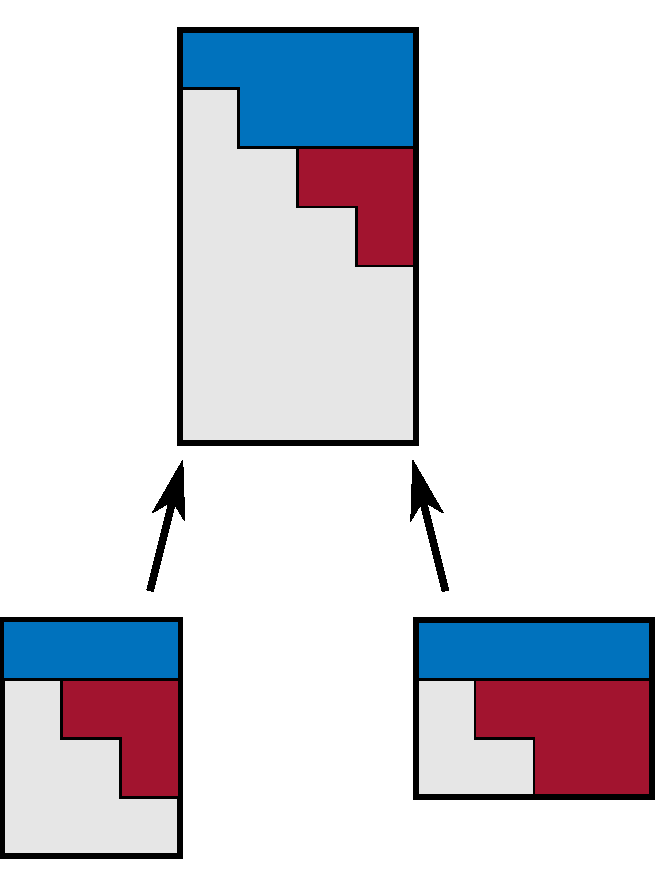
\includegraphics[width=0.5\textwidth]{figures/tree}}
    \only<2>{\includegraphics[width=0.5\textwidth]{figures/tree2}}
    \only<3>{\includegraphics[width=0.5\textwidth]{figures/tree3}}
  \end{center}

\end{frame}

\begin{frame}{STF vs PTG: Front partitioning}
    
    How can we adapt the front partitioning depending on the context of
    execution?

    \begin{itemize}

    \item \db{Node parallelism} at \alert{top of the tree} or when
      \alert{reaching a memory constraint}: fine grain partitioning
      \begin{itemize}
      \item more parallelism
      \item better pipeline
      \end{itemize}
    \end{itemize}      

  \begin{center}
    \only<1>{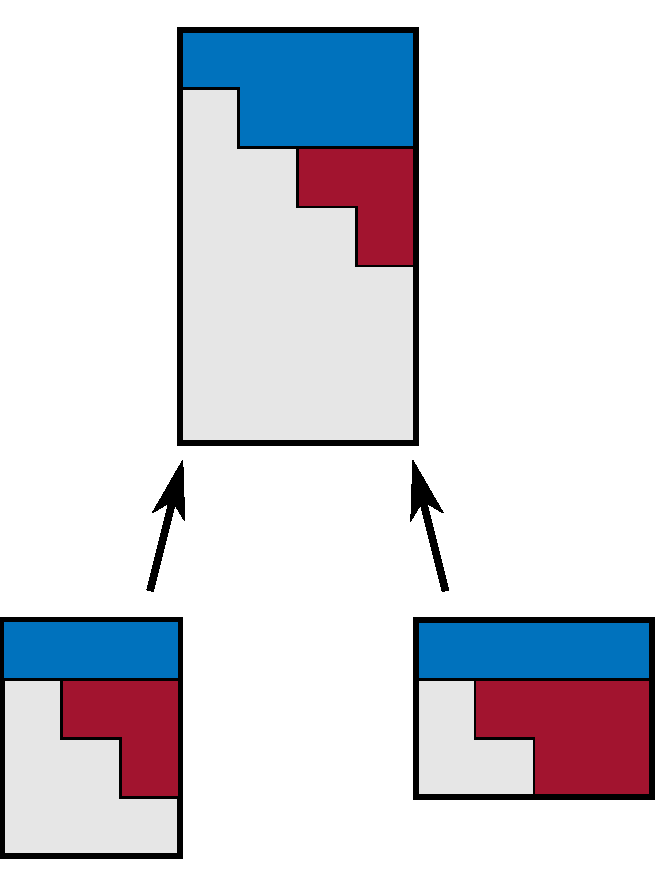
\includegraphics[width=0.5\textwidth]{figures/tree}}
    \only<2>{\includegraphics[width=0.5\textwidth]{figures/tree4}}
    \only<3>{\includegraphics[width=0.5\textwidth]{figures/tree5}}
  \end{center}

\end{frame}

\begin{frame}{STF vs PTG: Front partitioning}
    
    How can we adapt the front partitioning depending on the context of
    execution?

    \begin{itemize}
    \item Extremely challenging to apply these rules in practice:
      \begin{itemize}
      \item Huge search space for parameters 
        \begin{itemize}
        \item Tile dimensions
        \item Inner blocking sizes
        \item Panel reduction trees
        \end{itemize}
      \item Take into account the sparse structure of frontal matrices
        (staircase structure)
      \end{itemize}
    \end{itemize}

\end{frame}

%% \begin{frame}[plain]{Heterogeneous systems}

%%   \db{Dynamic} approach with qrm\_parsec vs \db{static} approach with
%%   qrm\_starpu:

%%   \begin{columns}
%%     \begin{column}{0.5\textwidth}
      
%%       In \db{qrm\_starpu}:
%%       \begin{itemize}
%%       \item Multilevel block partitioning: fine-grained task for CPUs and
%%         large-grained task for GPUs
%%         %% \item Tasks are scheduled to their granularity  
%%       \end{itemize}

%%       In \db{qrm\_parsec}:
%%       \begin{itemize}
%%       \item Fixed block partitioning with large blocks: large-grained task
%%         for GPUs. 
        
%%         \alert{On CPUs?} split tasks into fine granularity tasks
%%         %% \item Tasks are scheduled to their granularity  
%%       \end{itemize}
%%     \end{column}
%%     \begin{column}{0.5\textwidth}

%%       \begin{center}
%%         \includegraphics[width=0.8\textwidth]{figures/mlb}
%%       \end{center}
%%     \end{column}
%%   \end{columns}

%% \end{frame}

%% \begin{frame}[plain,fragile]{2D partitioning + CA front factorization}
%% \begin{lstlisting}[basicstyle=\tt\tiny]
%% do f=1, nfronts                                  ! in sequential order
%%   call starpu_submit(activate, f)                ! activate front
%%   call starpu_submit(init, f)                    ! init front

%%   do c=1, f%nchildren                            ! for all the children of f
%%     do i=1,c%m
%%       do j=1,c%n
%%         call starpu_submit(assemble, c, i, j, f) ! assemble block(i,j) of c into f
%%       end do
%%     end do
%%     call starpu_submit(deactivate, c)            ! Deactivate child
%%   end do

%%   ca_facto: do k=1, min(f%m,f%n)
%%     do s=0, log2(f%m-k+1)
%%       do i = k, f%n, 2**s
%%         if(s.eq.0) then
%%           call starpu_submit(geqrt, f, k, i)
%%           do j=k+1, f%n
%%             call starpu_submit(gemqrt, f, k, i, j)
%%           end do
%%         else
%%           l = i+2**(s-1)
%%           call starpu_submit(tpqrt, f, k, i, l)
%%           do j=k+1, front%n
%%             call starpu_submit(tpmqrt, f, k, i, l, j)
%%           end do
%%         end if
%%       end do
%%     end do
%%   end do ca_facto
%% end do
%% call starpu_waitall()                         ! wait for the tasks to be executed
%% \end{lstlisting}

%% \end{frame}


% \part{Experimental results}

% \begin{frame}[plain]
%   \partpage
% \end{frame}


% \begin{frame}{Experimental results}
%   \begin{columns}
%     \begin{column}{0.5\textwidth}

%       \texttt{\tiny
%         \begin{tabular}{rlrl}
%           \hline
%           \# & Matrix             & Gflops & Ordering  \\
%           \hline
%           1  & EternityII\_A      & 43     & COLAMD  \\
%           2  & LargeRegFile       & 80     & COLAMD  \\
%           3  & sc205-2r           & 101    & COLAMD  \\
%           4  & cont11\_l          & 162    & COLAMD  \\
%           5  & scagr7-2r          & 209    & COLAMD  \\
%           6  & tp-6               & 245    & COLAMD  \\
%           7  & karted             & 247    & COLAMD  \\
%           8  & EternityII\_Etilde & 467    & COLAMD  \\
%           9  & EternityII\_E      & 530    & COLAMD  \\
%           10 & degme              & 574    & COLAMD  \\
%           11 & cat\_ears\_4\_4    & 682    & COLAMD  \\
%           12 & hirlam             & 2123   & COLAMD  \\
%           13 & e18                & 3291   & COLAMD  \\
%           14 & flower\_7\_4       & 3725   & COLAMD  \\
%           15 & Rucci1             & 12351  & COLAMD  \\
%           16 & sls                & 22014  & COLAMD  \\
%           17 & TF17               & 37400  & COLAMD  \\
%           18 & spal\_004          & 59787  & COLAMD  \\
%           \hline
%           19 & hirlam             & 1384   & SCOTCH  \\
%           20 & flower\_8\_4       & 2851   & SCOTCH  \\
%           21 & Rucci1             & 5772   & SCOTCH  \\
%           22 & sls                & 65607  & SCOTCH  \\
%           23 & TF17               & 12416  & SCOTCH  \\
%           24 & spal\_004          & 30335  & SCOTCH  \\
%           25 & TF18               & 194660 & SCOTCH  \\
%           \hline
%         \end{tabular}}
%     \end{column}
%     \begin{column}{0.5\textwidth}
%       \begin{itemize}
%       \item {\bf System 1}:
%         \begin{itemize}
%         \item IBM x3755
%         \item AMD Opteron Processor 8431 @ 2.4 GHz, $4\times
%           6$ cores
%         \item 72 GB memory (NUMA)
%         \end{itemize}

%       \item {\bf System 2}:
%         \begin{itemize}
%         \item IBM x3750-M4
%         \item Intel Sandy Bridge E5-4650 @ 2.7
%           GHz, $4\times 8$ cores
%         \item 128 GB memory (NUMA)
%         \end{itemize}
%       \end{itemize}
%     \end{column}
%   \end{columns}

% \end{frame}

%% \begin{frame}{Experimental results: System 1}
%%   \begin{center}
%%     \only<1>{\includegraphics[width=\textwidth]{data/su_1d_2d_1} }
%%     \only<2>{\includegraphics[width=\textwidth]{data/su_1d_2d_2} }
%%   \end{center}
%% \end{frame}

%% \begin{frame}{Experimental results: System 1}
%%   \begin{center}
%%     \includegraphics[width=\textwidth]{data/breakdown}
%%   \end{center}
%% \end{frame}

%% \begin{frame}{Experimental results: System 2}
%%   \begin{columns}
%%     \begin{column}{0.4\textwidth}
%%       \texttt{\tiny
%%         \begin{tabular}{rlrl}
%%           \hline
%%           \# & Matrix             & Gflops & Ordering  \\
%%           \hline
%%           19 & hirlam             & 1384   & SCOTCH  \\
%%           20 & flower\_8\_4       & 2851   & SCOTCH  \\
%%           21 & Rucci1             & 5772   & SCOTCH  \\
%%           22 & sls                & 65607  & SCOTCH  \\
%%           23 & TF17               & 12416  & SCOTCH  \\
%%           24 & spal\_004          & 30335  & SCOTCH  \\
%%           25 & TF18               & 194660 & SCOTCH  \\
%%           \hline
%%         \end{tabular}}

        
%%         \vspace{0.5cm}
        
%%         \small
%%         {\bf System 2}:
        
%%         \begin{itemize}
%%         \item IBM x3750-M4
%%         \item Intel Sandy Bridge E5-4650 @ 2.7
%%           GHz, $4\times 8$ cores
%%         \item 128 GB memory (NUMA)
%%         \end{itemize}
        

%%     \end{column}
%%     \begin{column}{0.6\textwidth}
%%       \begin{center}
%%         \includegraphics[width=\textwidth]{data/su_1d_2d_ada}
%%       \end{center}
%%     \end{column}
%%   \end{columns}
%% \end{frame}



%% \part{Memory aware parallelization}


%% \begin{frame}[plain]
%%   \partpage
%% \end{frame}

%% \begin{frame}{Memory consumption in multifrontal methods}

%%   \begin{block}{Memory in the multifrontal}
%%     \begin{itemize}
%%     \item the \alert{activate} routine allocates memory for the factors and for temporary data
%%     \item temporary data of a front is deallocated when its parent is
%%       activated and the node \alert{deactivated}
%%     \item factors are persistent in memory
%%     \end{itemize}
%%   \end{block}

%%   \vspace{0.5cm}

%%   Therefore the memory consumption
%%   \begin{itemize}
%%   \item \alert{varies} throughout the factorization
%%   \item depends on the specific different tree \dg{traversals}
%%   \item is generally increased by \db{parallelism}
%%   \end{itemize}
%% \end{frame}


%% \begin{frame}{Memory consumption in multifrontal methods}
%%   \begin{center}
%%     \only<1>{\includegraphics[width=0.9\textwidth]{figures/ma_anim1} }%
%%     \only<2>{\includegraphics[width=0.9\textwidth]{figures/ma_anim2} }%
%%     \only<3>{\includegraphics[width=0.9\textwidth]{figures/ma_anim3} }%
%%     \only<4>{\includegraphics[width=0.9\textwidth]{figures/ma_anim4} }%
%%   \end{center}
%%   \begin{itemize}
%%   \item<2-> an eager scheduling may almost instantly activate all the fronts
%%   \item<3-> how much concurrency with the sequential memory peak?
%%   \item<4-> how much concurrency within an imposed memory bound?
%%   \end{itemize}
%% \end{frame}


%% \begin{frame}[fragile,t,plain]{Memory aware scheduling in a STF model}
  
%%   \vspace{-0.2cm}

%% \begin{lstlisting}[basicstyle=\tt\tiny]
%% do f=1, nfronts                                  ! in sequential order

%%   call starpu_submit(activate, f)                ! avail_mem -= size(f)
%%   call starpu_submit(init, f)                    ! init front

%%   ...

%%   ! front assembly
%%   ...
%%     call starpu_submit(deactivate, c)            ! avail_mem += size(temp_f)
%%   ...        

%%   ! front factorization
%%   ...

%% end do
%% call starpu_waitall()                            ! wait for the tasks to be executed
%% \end{lstlisting}

%% \end{frame}


%% \begin{frame}[fragile,t,plain]{Memory aware scheduling in a STF model}
  
%%   \vspace{-0.2cm}

%% \begin{lstlisting}[basicstyle=\tt\tiny]
%% do f=1, nfronts                                  ! in sequential order
%%   do while(avail_mem < size(f)) wait()
%%   call starpu_submit(activate, f)                ! avail_mem -= size(f)
%%   call starpu_submit(init, f)                    ! init front

%%   ...

%%   ! front assembly
%%   ...
%%     call starpu_submit(deactivate, c)            ! avail_mem += size(temp_f)
%%   ...

%%   ! front factorization
%%   ...

%% end do
%% call starpu_waitall()                            ! wait for the tasks to be executed
%% \end{lstlisting}


%%   How to impose a memory constraint:
%%   \begin{itemize}
%%   \item Subordinate the activation of a front and the submission of
%%     the related tasks to the availability of memory
%%   % \item \phantom{Execute the activation routines in exactly the same order as
%%     % in sequential: this ensures that no memory deadlocks happen
%%     % (related to deadlock avoidance methods by Dijkstra, EWD-108, early 60s)}
%%   \end{itemize}

%% \end{frame}

%% \begin{frame}[fragile,t,plain]{Memory aware scheduling in a STF model}
  
%%   \vspace{-0.2cm}

%% \begin{lstlisting}[basicstyle=\tt\tiny]
%% do f=1, nfronts                                  ! in sequential order
%%   do while(avail_mem < size(f)) wait()
%%   call activate(f)                               ! avail_mem -= size(f)
%%   call starpu_submit(init, f)                    ! init front

%%   ...

%%   ! front assembly
%%   ...
%%     call starpu_submit(deactivate, c)            ! avail_mem += size(temp_f)
%%   ...

%%   ! front factorization
%%   ...

%% end do
%% call starpu_waitall()                            ! wait for the tasks to be executed
%% \end{lstlisting}


%%   How to impose a memory constraint:
%%   \begin{itemize}
%%   \item Subordinate the activation of a front and the submission of
%%     the related tasks to the availability of memory
%%   \item Execute the activation routines in the same order as
%%     in sequential: this ensures no memory deadlocks happen
%%     (deadlock avoidance methods by Dijkstra, EWD-108, early 60s)
%%   \end{itemize}

%% \end{frame}


%% \begin{frame}{Experimental results}
%%   \begin{center}
%%     \includegraphics[width=\textwidth]{data/ma}
%%   \end{center}
%% \end{frame}

\newcommand{\gargantuan}{\fontsize{250}{250}\selectfont}

\part{Conclusions and future work}

\begin{frame}[plain]{Conclusions and future work}
  %% \small
  %% \begin{block}{Objective}
  %%   Develop a PaRSEC version of \qrm following the \alert{PTG model} and
  %%   evaluate its effectiveness on a single-node, multicore systems
  %% \end{block}

  \begin{block}{Conclusions on PaRSEC}
    %% \vspace{-0.3cm}

    \begin{itemize}
    \item More challenging to use than other runtimes systems
    \item Potentially more scalable
    \item Some features should be added PaRSEC to enhance the current
      version of qr\_parsec
    \end{itemize}
    
  \end{block}

  \begin{block}{Ongoing and Future work}
    \begin{itemize}
    \item Use GPUs with PaRSEC   
    \item Distributed-memory architecture  
    \end{itemize}
  \end{block}
  
  

\end{frame}

%% \begin{frame}[plain]
%%   \partpage
%% \end{frame}

%% \begin{frame}[plain]{Conclusions and future work}


%%   \small
%%   \begin{block}{Conclusions}

%%     \vspace{-0.3cm}

%%     \begin{itemize}
%%     \item In the etree the parent-child dependencies are not finely
%%       managed resulting lower pipeline efficiency in the case of qrm\_parsec 
%%     \item 
%%     \item Modern runtime engines are efficient and introduce a small
%%       (almost insignificant) overhead
%%     \end{itemize}
%%   \end{block}

%%   \begin{exampleblock}{Ongoing and future work}

%%     \vspace{-0.3cm}

%%     \begin{itemize}
%%     \item port to accelerators (ongoing)
%%     \item evaluate other runtimes with other programming models such
%%       as Parametrized Task Gragh (ongoing, with G. Bosilca)
%%     \item data-locality scheduling with contexts (ongoing, with A. Hugo)
%%     \item memory-aware traversals (ongoing with L. Marchal et al.)
%%     \end{itemize}
%%   \end{exampleblock}
%% \end{frame}

\begin{frame}[plain]{}
  \begin{beamercolorbox}[wd=\paperwidth, ht=\paperheight, sep=15pt]{block title}%

    \vspace{-20cm}

    \begin{columns}
      \begin{column}{0.2\textwidth}

        \vspace{-2cm}

        \hspace{1cm}  {\gargantuan ?}
      \end{column}
      \begin{column}{0.8\textwidth}

        \vspace{-2cm}

        \vspace{0.3cm}

        {\huge Thanks for the welcome at ICL!}

        {\huge Questions?}

      \end{column}
    \end{columns}

    %% {\Huge Thanks for the Welcome at ICL!}

  \end{beamercolorbox}

  \vspace{2cm}

\end{frame}



\end{document}
